\section{Electrical Design}
\label{sec:electrical_design}

In this module, the following will be discussed:
\begin{itemize}
\item Subsystem Description
\item Requirements
\item Tests and Results, Future Test Plans
\item Design Modifications
\item Compatibility Analysis
\end{itemize}

\subsection{Subsystem Description}
In this subsystem, all electronic components are connected and powered up for the use of other subsystems. The subsystem contains batteries, voltage regulators, battery chargers, relays, diodes, a microcomputer, a micro-controller and a servo motor. Flowchart of this subsystem is shown in Figure \ref{fig:flowelec}. 
%bu flowchart kotu oldu=?

\begin{figure}[h!]
     \centering
     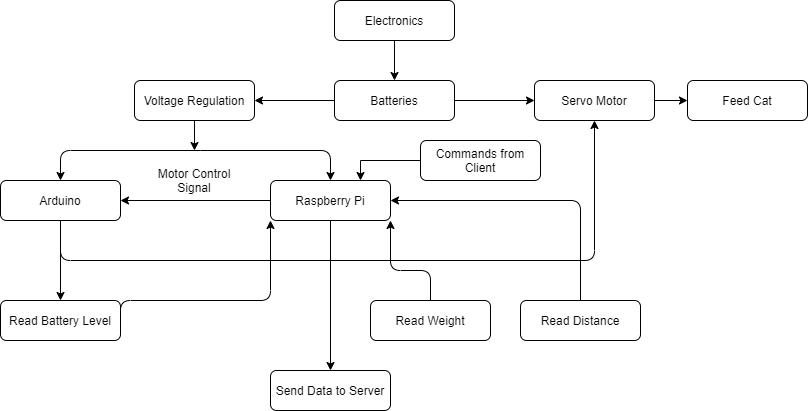
\includegraphics[width=1.1\columnwidth]{content/050_electrical_design/elektronikflow.png}
     \caption{ Flowchart of the Electronics Subsystem}
     \label{fig:flowelec}
\end{figure}

\subsubsection{Supply Unit} 

Supply connections for the motor and controller units are shown in Figure \ref{fig:elecdesign}.
Two separate battery units are designed for motor and controller units to obtain better motor performance. 

High motor torque is required for the rotation of the mechanical gate. 2 Lithium-Ion Batteries are connected in series to obtain a voltage in the input voltage range of the MG996R servo motor. Parallel and series combination of diodes are added at the end of this unit. Parallel diodes increase the maximum passing current of the node, and serial diodes are used to keep the voltage in the input range. Relays are added to decrease power consumption and increase charging speed. The relays RL1 and RL2 shown in \ref{fig:elecdesign} are used for parallel charging operation while the outer box is connected to the power outlet with a micro-USB adapter. Also, while the box is not plugged in, the batteries become serially connected, as explained above. However, in this way, the motor is not able to operate during the charging operation. Another relay RL3 is added to solve this problem. The power of the motor is supplied directly from the power outlet during the charging operation, and it is supplied from the batteries while the box is not plugged in. Furthermore, the relay RL4 is connected to decrease power consumption. It is controlled from the Raspberry Pi and turns on the motor when a cat is detected.

For Raspberry Pi and Arduino, a constant stable voltage input is required, so a 5V step up voltage regulator is used. Two Lithium-Ion batteries are connected in parallel to increase usage time and the batteries are directly connected to the step up voltage regulator. Both Raspberry and Arduino are supplied from this regulator.

For charging operation, 3 different charger circuits are connected parallelly as seen from the Figure \ref{fig:elecdesign} and all batteries are charged up synchronously.

Also, two resistors are used to read analog voltages from the Arduino.


\begin{figure}[H]
     \centering
     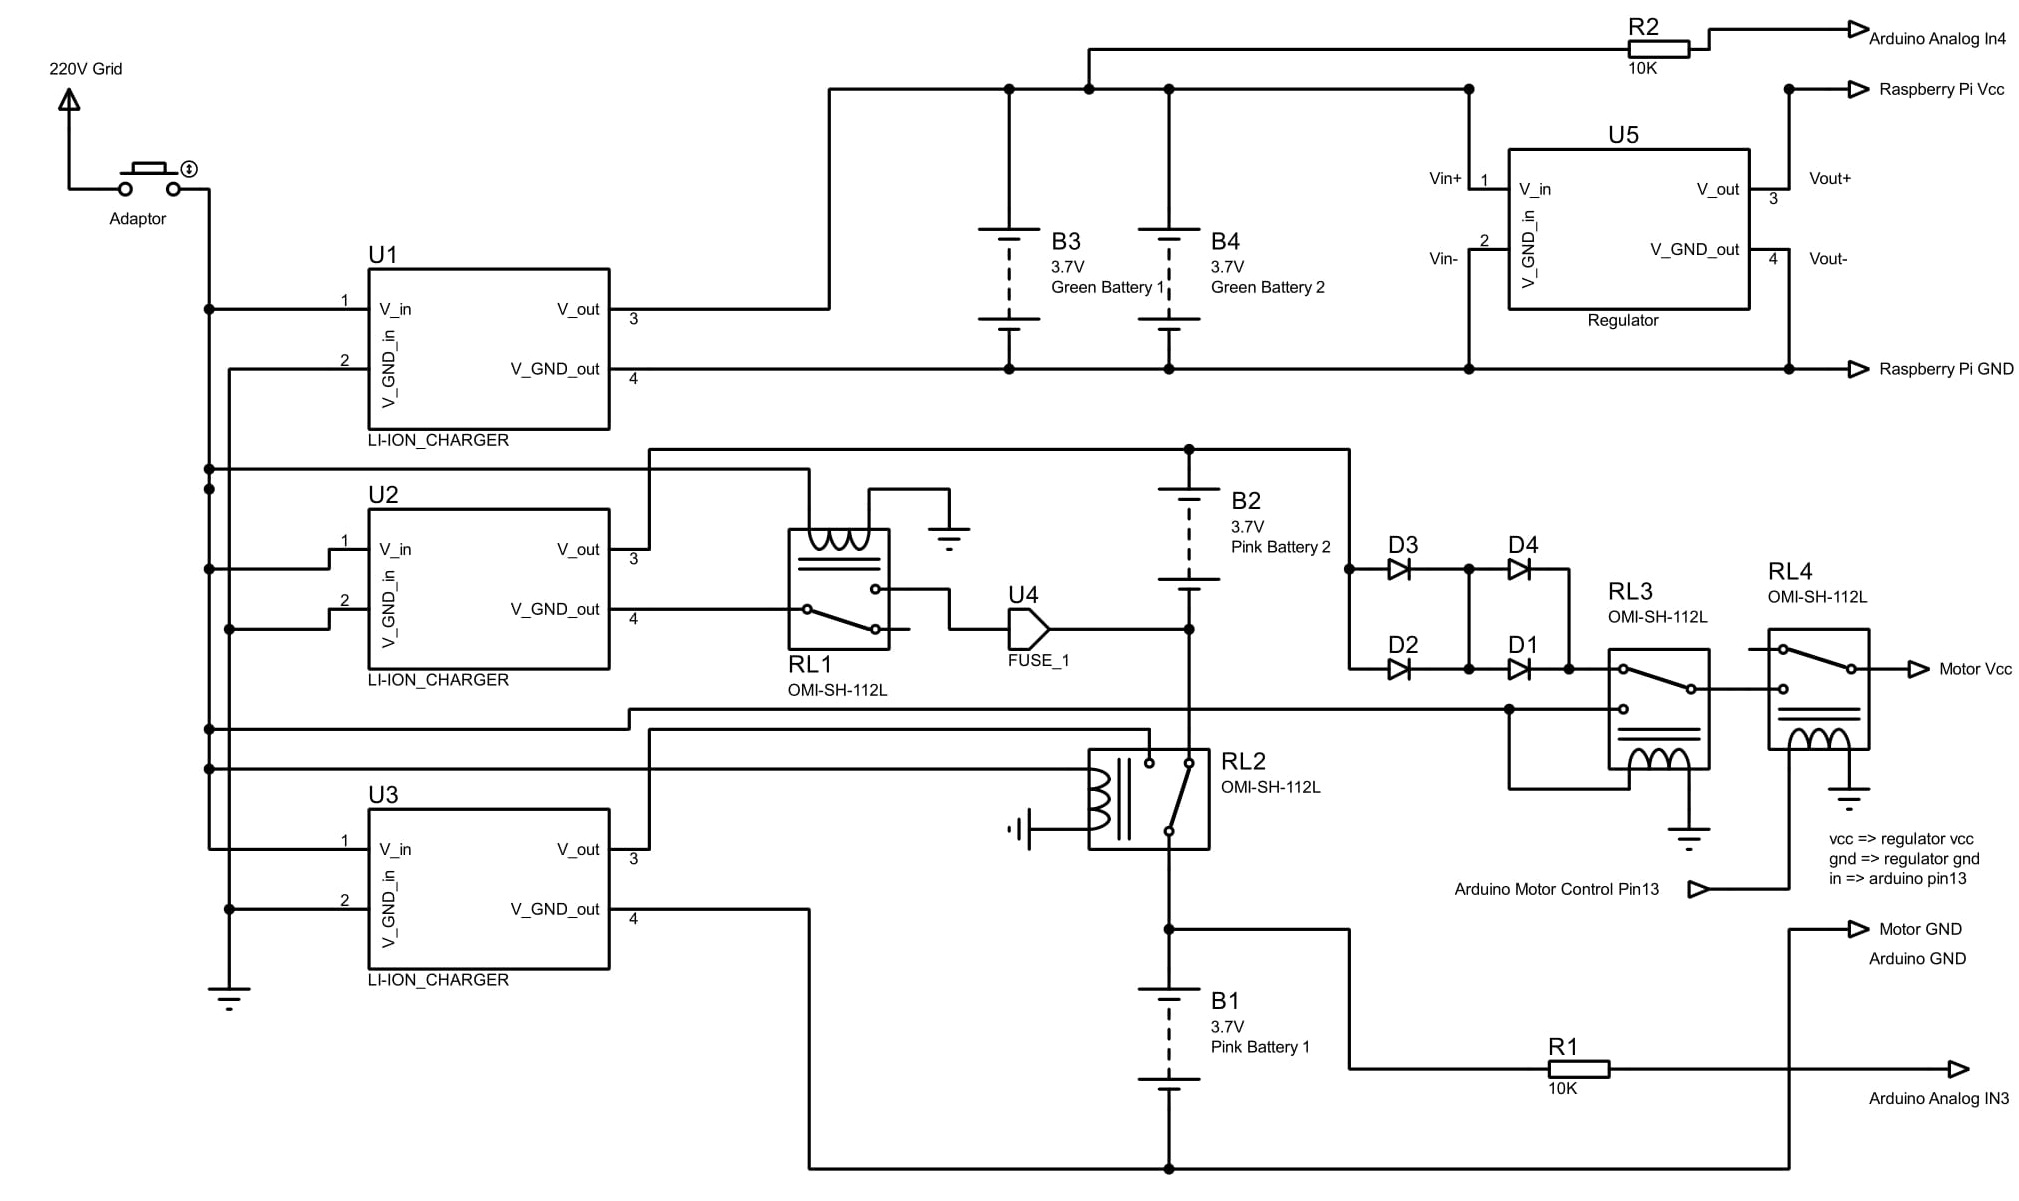
\includegraphics[width=1.3\columnwidth, angle=90]{content/050_electrical_design/Design_V2-1.jpg}
     \caption{ Circuit Design of the Supply Unit}
     \label{fig:elecdesign}
\end{figure}


\subsubsection{Raspberry Pi and Arduino} 
Raspberry Pi is the main control mechanism of the project and its operations are listed below.

\begin{itemize}
\item Receiving images from the camera module and transferring them to the server.
\item Controlling the rotation of the motor by sending a control signal to Arduino through a serial communication channel, and this command opens the Relay 5 shown in Figure \ref{fig:elecdesign} and generates a PWM signal.
\item Measuring the distance coming from the ultrasonic sonar sensor, converting the measurement to volume, and sending it to the server.
\item Measuring the weight of the given food and sending the data to the server.
\item Receiving the analog battery voltages from the Arduino by using I2C serial communication protocol to indicate battery level in the web interface.
\item Controlling the LEDs which indicate the detection of cats/dogs.
\item Controlling the operation of the light bulb according to the time.

\end{itemize}
Arduino is the second controller used in the project and its operations are listed below.
\begin{itemize}
\item  Controlling the servo motor by generating PWM signals when rotation command is received from Raspberry Pi.
\item Receiving the analog voltage data from the batteries and transmitting the data to the Raspberry Pi.
%\item Gece görüşü lambası ???? %%%%%%%%%%
\end{itemize}

\subsubsection{Servo Motor} 
Servo motor rotates the food gate according to the amount of food calculated for each different cat, and it is controlled by changing the duty cycle of the PWM signal generated in Arduino. The motor unit is explained in more detail in the mechanical design part of this report. 

\subsubsection{Measuring the Food Level}

The users are informed about the remaining food level in the reservoir. The food level is measured by the ultrasonic sonar sensor HC-SR04, which measures the distance between the food and sensor. The sensor generates an ultrasonic sound around 40kHz, and the amplitude of this sound is very low in order not to disturb the animals. The sensor contains two different transducers. The first transducer generates the sound wave, and the second transducer receives the echo of the transmitted wave. The distance is calculated by the following formula:

\begin{equation}
\text{distance = time $\times$ speed of sound  /  2}
\end{equation} % ;) :*

The generated sound is transmitted from the transducer, and then the wave bounces back from the object; the returned wave is received from the second transducer. The distance is divided by 2 since the sound makes a round trip between the sensor and the food. Sound speed is taken as 340 meters per second. The measured distances are proportioned with respect to the reference level, and volume measurement is obtained.


\subsubsection{Measuring the Weight}
  
A weight sensor is used in order to obtain the amount of food given to the cats.  The sensor has three input wires. The sensor returns analog voltage values with respect to the applied force on the sensor. This analog voltage should be converted into digital data. An analog to digital converter HX711 integrated circuit is used, and the digital data is read through a port in the raspberry pi and scaled according to the measured weights.



\subsection{Requirements}
The requirements for the electronics subsystem are listed below.
\begin{itemize}
\item The subsystem should be rechargeable and the charging time should be less than 5 hours.
\item Rechargeable batteries should be non-removable.
\item Battery duration should be at least 5 hours.
\item The subsystem should be wired correctly and properly.
\item The subsystem should be able to operate during charging.
\item The subsystem should be able to operate Raspberry Pi and Arduino.
\item The subsystem should be able to drive the servo motor.
\item Power consumption of the subsystem should be minimum. % not measurable
\item Status of the food supply should be observable.
\item Battery level for both charging and operation modes should be observable.
\item The subsystem should be able to measure the amount of given food.

\end{itemize}




\subsection{Tests and Results, Future Test Plans}

\subsubsection{Test Procedure}
  
%Test Procedure is explained below.
\begin{itemize}
\item Measure the voltage of batteries.
\item Charge the batteries with charger circuits until the voltages are balanced.
\item Connect batteries to regulators.
\item Measure the output voltage of regulators for different voltages inside the voltage range of battery.
\item Connect relays.
\item Power up the Raspberry Pi, Arduino, and the motor.
\item Connect all sub-units properly.
\item Measure the distance with sonar sensor.
\item Measure the weight of given food.
\item Drive the motor.
\item On-Off control of the light bulb.
\item Obtain images from the camera.
\item Measure the maximum and minimum camera view distance.
\item Drive the motor while camera is active.
\item Measure the distance while motor and camera are active.
\item Measure the weight while distance sensor, motor and camera are active.
\item Measure the currents for power analysis.
\end{itemize}


\subsubsection{Test Results} 
\begin{itemize}
\item Li-Ion batteries operates properly. Output voltage is between 3.7V and 4.2V.
\item Parallel charging for two different power supply units with 3 charger operates correctly.
\item Batteries work while charging. The subsystem requirement for re-chargeability is satisfied. 
\item 5V 1.2A regulators return 5.35Volts when the  input is 3.7V  and 5.45 Volts when the input is 4.2V.  This is undesired, however does not cause any faults or performance loss for the operation of raspberry pi and arduino.
\item Relays work correctly.
\item All connections are done in a board and placed in a fixed layer. For charging operation, a micro-USB socket is placed outside of the box. Thus, the subsystem requirement for non-removable batteries is satisfied. Also, solders and connectors are used in wiring, and cable connections are optimized and hidden.
\item Raspberry Pi, Arduino and Motor operates without a performance loss.
\item Measured distances are correct if the distances are away from the sensor 2 centimeters and results are shown in Figure ~\ref{fig:sonardist}.

\begin{figure}[h!]
     \centering
     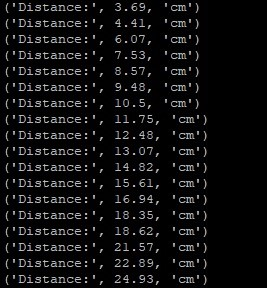
\includegraphics[width=0.45\linewidth]{content/050_electrical_design/sonardistance-1.jpg}
     \caption{ Measured Distances From Ultrasonic Sonar Sensor}
     \label{fig:sonardist}
\end{figure}



\item Weight sensor does not read small values, a better resolution sensor will be implemented.
\item Motor is rotated according to the entered amount of food properly. Generated PWM signals can be seen in Figure~\ref{fig:pwmaaa}.
\begin{figure}[ht]
     \centering
     \begin{subfigure}[b]{0.49\textwidth}
     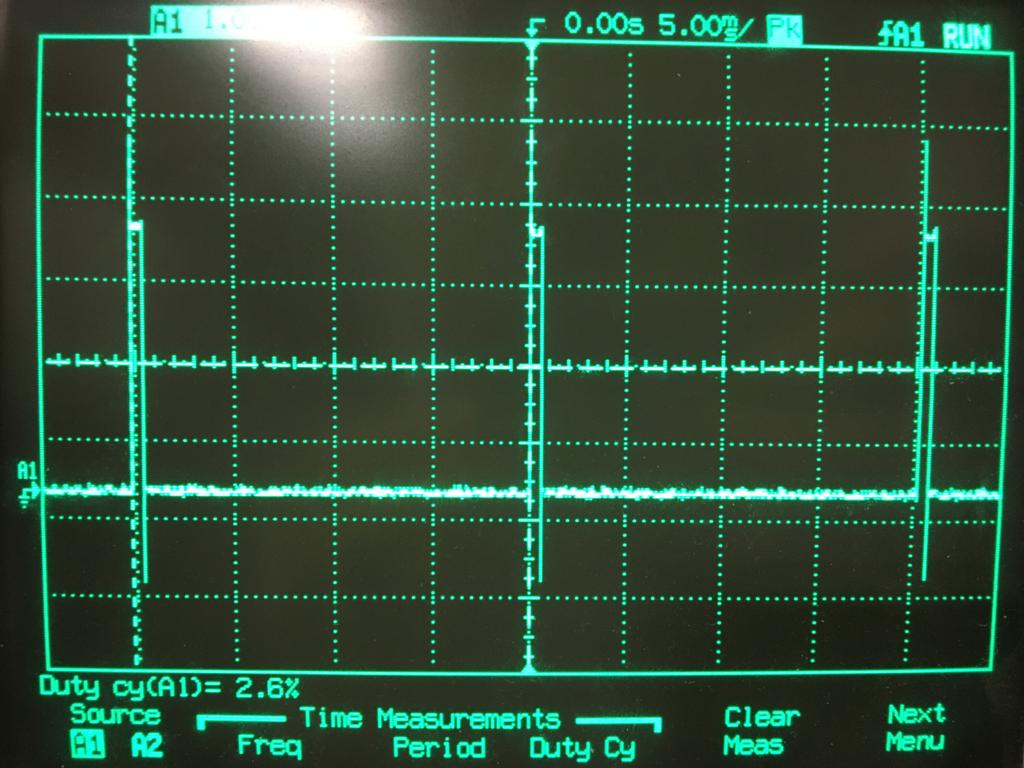
\includegraphics[width=\linewidth]{content/050_electrical_design/pwm25.jpeg}
     \caption{PWM Signal Duty Cycle = 2.5}
     \label{fig:pwm25}
     \end{subfigure}
     \begin{subfigure}[b]{0.49\textwidth}
     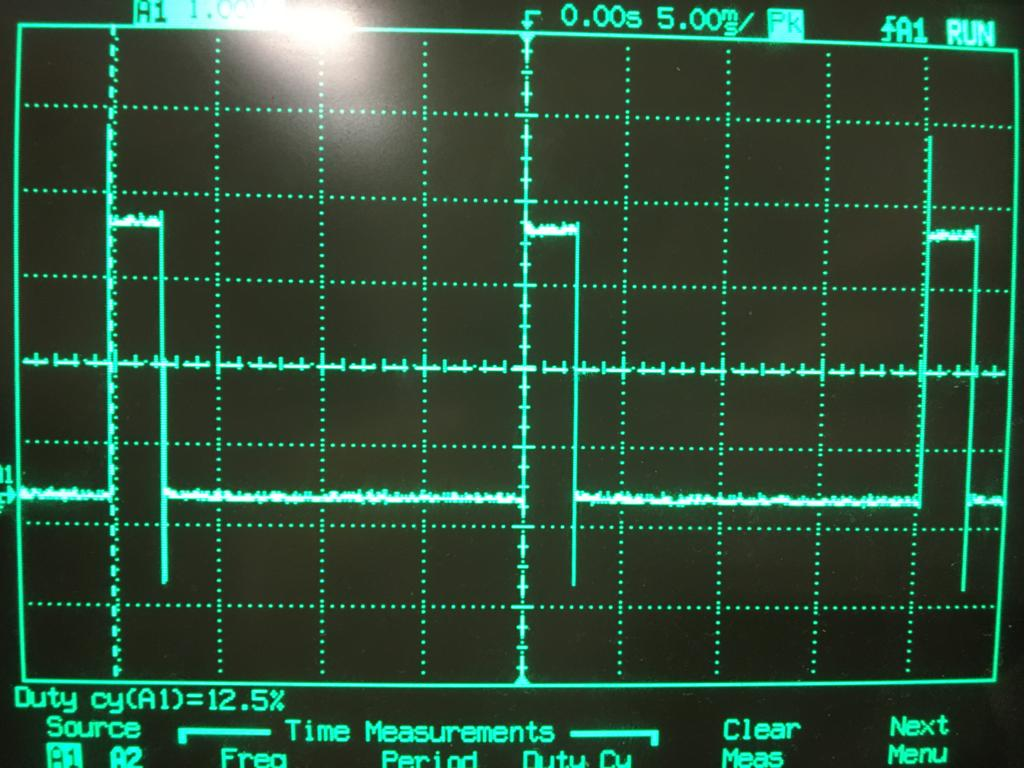
\includegraphics[width=\linewidth]{content/050_electrical_design/pwm125.jpeg}
     \caption {PWM Signal Duty Cycle = 12.5}
     \label{fig:pwm125}
     \end{subfigure}        
     \caption{Generated PWM signals from the Raspberry Pi}
     \label{fig:pwmaaa}
\end{figure}
\item High quality images are obtained.
\item A dog can be detected from the taken image from the camera with a distance range of 10 cm to 180 cm away from the box. Average detection distance is 110cm. 
\item A cat can be detected from the taken image from the camera with a distance range of 15 cm to 153 cm away from the box.
\item The system operates properly while motor and all sensors are working. The jittering issue mentioned in the conceptual design report is solved.
\item The battery unit draws 0.84 A when they are fully discharged. Charging and operation times are mentioned in the power analysis section of the report.
\item Currents are measured and written in the power analysis section of the report. The drawn currents for the units are reduced by using relays and power consumption is decreased.
\end{itemize}




\subsection{Modifications}

According to the test results, some modifications are applied to the system, as listed below.
\begin{itemize}
\item Fuses are added to obtain a safer system. 
\item Motor noise is eliminated. In the previous design, the motor is driven from raspberry pi, and raspberry generates an unstable PWM signal while the camera is operating. Arduino UNO is implemented in the system to obtain a stable PWM signal. The command still comes from the raspberry pi, and it is transmitted to Arduino by a serial communication channel using I2C communication protocol.  When the command arrives arduino in milliseconds, the motor rotates properly. 
\item Relays are added to reduce power consumption and get rid of adjustable voltage regulator. The relay connections are shown in Figure\ref{fig:elecdesign}. 
\begin{itemize}
\item Adjustable voltage regulator did not work properly due to an increase in its temperature. We used relays and got rid of this regulator. The relays RL1, RL2, and RL3 are used for this purpose. Servo motor MG996R operates in the voltage range between 4.8 V and 7.2V, and out batteries supply voltage in the range 3.7V-4.2V.  We find a solution with 3 relays and 4 diodes for this problem.  While the motor is supplied the batteries, two batteries are connected in series supplying 8.2V, this voltage is reduced 1.4 Volts by connecting series added diodes. Two parallel connected diodes are connected in series with another parallel connected diodes. Thus, voltage is reduced by 1.4 volts, and the motor can get the required current from the batteries. For charging circuit, relay1 and relay2 are switched and the series connected batteries are isolated. Batteries are charged separately, and with relay RL3, the motor supply is also switched and motor is supplied from the power outlet.
\item Relay RL4 shown in  Figure\ref{fig:elecdesign} is connected to reduce power consumption. The motor supply connections are turned of with this relay until a turn on command comes from the raspberry pi.
\end{itemize}
\end{itemize}

\subsection{Compatibility Analysis}

It is observed that the electronics system is reliable when it is connected with the other systems. All systems operate at the required performance and no error is observed. Although the system is working properly, the control mechanism of the motor will be calibrated according to the feeding regimes of the cats. Also, time calibration will be done for the light bulb. However, at some nodes, the long cabling might decrease the performance of sub-units when the inner design is placed in the outer box. If this situation occurs, cable connections will be re-arranged.

